\chapter{Test and evaluation}
In this chapter, we will discuss how the testing is done
in the implementation of this work as well as how
the current model was evaluated.
\section{Test}
In the current implementation, we test our prototype by the means
of unit testing. Unit testing is a method of software testing,
which verifies that individual units of the code are working
as expected. To perform the unit testing, one should identify
pieces of code, that are responsible for a clear task \cite{Huizinga2007}.
In most cases,
that are methods of classes or functions. Imagine, that we have
a function that adds two numbers together. To test this function,
we have to come up with the real values, calculate the expected
return, call the function with the real value and compare
the return of the function with the expected return:

\begin{lstlisting}[language=Python, caption={TensorFlow example \cite{tensorflow2015-whitepaper}},label={list:test_ex}]

	def add(x, y):
		"""Add two numbers together."""
		return x + y

	# unit test of the function `add`
	def test_add():
		assert add(3, 5) == 8 # 3, 5 are real values, 8 is the expected return
		assert add(10, 2) == 12
\end{lstlisting}

In case of classes, mostly it's methods were covered with unit tests.
For testing purposes, we
used unit test framework called Nose. Nose simplifies unit testing
by providing automatic test discovery. It also automatically creates a test suite,
which is nothing more than a set of tests. One advantage of using the Nose
over the Python’s standard unit test module is that no configuration is required
in order to run all tests when the tests are named consistent with Nose conventions
and are located in the \emph{/tests} directory. An additional advantage is that
Nose generates well-readable report after running tests. The report helps
when debugging and fixing tests. You can see the example of an report on the figure
\ref{fig:report_test}

% TODO: two figures from the command line
\begin{center}
	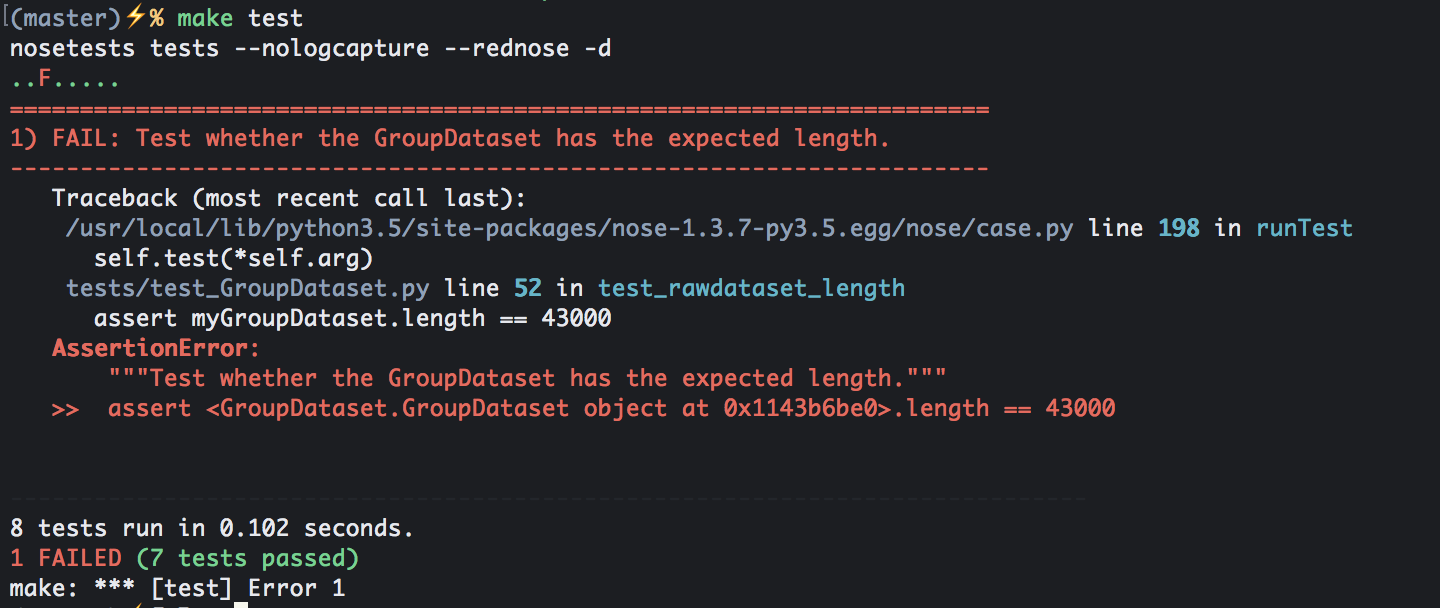
\includegraphics[width=\linewidth]{test_report}
	\caption{Output of executing command \lstinline{make test} in the root of the prototype
		with a failing test.
	}
	\label{fig:report_test}
\end{center}

\subparagraph{} The module Dataset is fully tested with unit tests. However,
the module Model is not, since it has too many non-deterministic values.
One good way of testing the model is to run an interactive session of TensorFlow,
which is desired for the further development of the prototype.\footnote{
TensorFlow documentation explains this method here: https://www.tensorflow.org/api\_guides/python/test
}

\section{Evaluation} The model was evaluated with the dataset described
in \autoref{sec:analysis_dataset} on server from HTW Berlin. The server
posses the Nvidia Tesla M40 GPU accelerator \cite{NVIDIA}.
It was required from 1 to 2 hours to train the model and the time is changed
caused by different configurations.
We will introduce more details of the first experiments below in this section.

\subsection{Configuration}
The evaluation was performed on three different types of setting.
You can see the differences between these configurations
in table \ref{tab:conf_exp}.

We will explain the settings that are different in the configurations:
\begin{itemize}
	\item Number of glimpses($T$) - As you can remember from \autoref{sec:ram_model}
	the agent does a classification decision after $T$ steps. In original RAM
	paper this number was equal to $T=7$. Since we will have more images in a group,
	we increased this number in all of configurations.
	\item Batch size - size of the batch for training the model.
	\item Labels of noise pictures - the images at the labels considered to be
	 	insignificant for the classification decision(as described in \autoref{sec:analysis_dataset}).
	\item Labels of non-noise pictures -  the image at the labels are important
		for the classification(as described in \autoref{sec:analysis_dataset}).

	\item Amount of images per group - this amount determines how many images
	a group will have.
	\item Amount of classes for classification task - as you may remember from
		\autoref{sec:analysis_dataset}, we can build dataset with different
		amount of classes.
\end{itemize}

\begin{table}[]
\centering
\resizebox{\textwidth}{!}{%
	\begin{tabular}{|l|l|l|l|}
	\hline
	Name of the parameter                     & Configuration 1        & Configuration 2           & Configuration 3           \\ \hline
	Batch size                                & 32                     & 20                        & 20                        \\ \hline
	Number of glimpses ($T$)                    & 30                     & 15                        & 24                        \\ \hline
	Labels of  noise pictures                 & 1,2                    & 0                         & 0                         \\ \hline
	Labels of non-noise pictures              & 0, 3, 4, 5, 6, 7, 8, 9 & 1, 2, 3, 4, 5, 6, 7, 8, 9 & 1, 2, 3, 4, 5, 6, 7, 8, 9 \\ \hline
	Amount of images per group                & 5                      & 5                         & 4                         \\ \hline
	Amount of classes for classification task & 3                      & 3                         & 2                         \\ \hline
	Amount of examples in training dataset    & 45000                  & 45000                     & 60000                     \\ \hline
	\end{tabular}
}
\caption{Configurations for the experiments}
\label{tab:conf_exp}
\end{table}

These configurations was a try to simplify the task for the model. From configuration 1
to configuration 3, we reduced training batch size, reduced the variety of the noise images,
reduced amount of classes, and played with number of glimpses.

\subparagraph{}
Of course, there even more parameters that is possible to tune
in further experiments. The explanation of all parameters can be found
in the implementation of the model.

\subsection{Results}
Generally speaking, the experiments highlighted that the model is not able
to generalise on the validation as well as on the test data.
We will show the evidence of that by referring to the figures taken from
TensorBoard.
The figures \ref{fig:valid_accuracy} and \ref{fig:test_accuracy} indicate that the accuracy on the validation
and test data weren't stable. The training accuracy for all three configurations
was stable and reached high results as shown in the figure \ref{fig:batch_accuracy}.
Proceeding from that, we can state that overfitting occurs
when training the model.

\begin{figure}
\centering
\begin{subfigure}{\textwidth}
  \centering
  \includegraphics[width=0.8\linewidth]{config1/batch_accuracy}
  \caption{Configuration 1}
  % \label{fig:b_acsub1}
\end{subfigure}
\begin{subfigure}{\textwidth}
  \centering
  \includegraphics[width=0.8\linewidth]{config2/batch_accuracy}
  \caption{Configuration 2}
  % \label{fig:sub2}
\end{subfigure}
\begin{subfigure}{\textwidth}
  \centering
  \includegraphics[width=0.8\linewidth]{config3/batch_accuracy}
  \caption{Configuration 3}
  % \label{fig:sub2}
\end{subfigure}
\caption{Accuracy on the training data}
\label{fig:batch_accuracy}
\end{figure}


\begin{figure}
\centering
\begin{subfigure}{\textwidth}
  \centering
  \includegraphics[width=0.75\linewidth]{config1/valid_accuracy}
  \caption{Configuration 1}
  \label{fig:sub1}
\end{subfigure}
\begin{subfigure}{\textwidth}
  \centering
  \includegraphics[width=0.75\linewidth]{config2/valid_accuracy}
  \caption{Configuration 2}
  \label{fig:sub2}
\end{subfigure}
\begin{subfigure}{\textwidth}
  \centering
  \includegraphics[width=0.75\linewidth]{config3/valid_accuracy}
  \caption{Configuration 3}
  \label{fig:sub2}
\end{subfigure}
\caption{Accuracy on the validation data}
\label{fig:valid_accuracy}
\end{figure}


\begin{figure}
\centering
\begin{subfigure}{\textwidth}
  \centering
  \includegraphics[width=0.75\linewidth]{config1/test_accuracy}
  \caption{Configuration 1}
  \label{fig:sub1}
\end{subfigure}
\begin{subfigure}{\textwidth}
  \centering
  \includegraphics[width=0.75\linewidth]{config2/test_accuracy}
  \caption{Configuration 2}
  \label{fig:sub2}
\end{subfigure}
\begin{subfigure}{\textwidth}
  \centering
  \includegraphics[width=0.75\linewidth]{config3/test_accuracy}
  \caption{Configuration 3}
  \label{fig:sub2}
\end{subfigure}
\caption{Accuracy on the test data}
\label{fig:test_accuracy}
\end{figure}

The figure \ref{fig:baseline_mse} shows that the mean squared error between our value function
for reducing the variance and actual reward is very small. This may indicate, that
the our baseline function is close to the actual expected reward.

Average reward value showed that agent was performing good and
in average was choosing the right actions. The evidence of that is
shown in the figure \ref{fig:average_reward}.
\begin{figure}
\centering
\begin{subfigure}{\textwidth}
  \centering
  \includegraphics[width=0.75\linewidth]{config1/test_accuracy}
  \caption{Configuration 1}
  \label{fig:sub1}
\end{subfigure}
\begin{subfigure}{\textwidth}
  \centering
  \includegraphics[width=0.75\linewidth]{config2/test_accuracy}
  \caption{Configuration 2}
  \label{fig:sub2}
\end{subfigure}
\begin{subfigure}{\textwidth}
  \centering
  \includegraphics[width=0.75\linewidth]{config3/test_accuracy}
  \caption{Configuration 3}
  \label{fig:sub2}
\end{subfigure}
\caption{Mean squared error between baseline function and expected reward}
\label{fig:baseline_mse}
\end{figure}

From the figure \ref{fig:hybrid_loss}, we can observe the hybrid loss value reduced much more in
the  configuration 3. The reason for this can be, that we reduced the amount
of classes from 3 to 2.
\begin{figure}
\centering
\begin{subfigure}{\textwidth}
  \centering
  \includegraphics[width=0.75\linewidth]{config1/hybrid_loss}
  \caption{Configuration 1}
  \label{fig:sub1}
\end{subfigure}
\begin{subfigure}{\textwidth}
  \centering
  \includegraphics[width=0.75\linewidth]{config2/hybrid_loss}
  \caption{Configuration 2}
  \label{fig:sub2}
\end{subfigure}
\begin{subfigure}{\textwidth}
  \centering
  \includegraphics[width=0.75\linewidth]{config3/hybrid_loss}
  \caption{Configuration 3}
  \label{fig:sub2}
\end{subfigure}
\caption{Hybrid loss}
\label{fig:hybrid_loss}
\end{figure}


\begin{figure}
\centering
\begin{subfigure}{\textwidth}
  \centering
  \includegraphics[width=0.75\linewidth]{config1/average_reward}
  \caption{Configuration 1}
  \label{fig:sub1}
\end{subfigure}
\begin{subfigure}{\textwidth}
  \centering
  \includegraphics[width=0.75\linewidth]{config2/average_reward}
  \caption{Configuration 2}
  \label{fig:sub2}
\end{subfigure}
\begin{subfigure}{\textwidth}
  \centering
  \includegraphics[width=0.75\linewidth]{config3/average_reward}
  \caption{Configuration 3}
  \label{fig:sub2}
\end{subfigure}
\caption{Average Reward}
\label{fig:average_reward}
\end{figure}


Broadly speaking, we found that it's required to
continue tuning the parameters of the model, as the figures clearly
highlighting the model's instability.
